% Draft for ICAART 2027 (regular paper). Layout approximates the SCITEPRESS
% two-column A4 format; port into the official template before submission.
\documentclass[10pt,a4paper,twocolumn]{article}
\usepackage[a4paper,left=1.9cm,right=1.9cm,top=2.6cm,bottom=2.6cm,columnsep=0.8cm]{geometry}
\usepackage{mathptmx}
\usepackage[T1]{fontenc}
\usepackage{amsmath,amssymb,amsthm}
\usepackage{graphicx,booktabs,multirow,xcolor}
\usepackage[hidelinks]{hyperref}
\hypersetup{pdfauthor={},pdftitle={},pdfsubject={},pdfkeywords={},pdfcreator={},pdfproducer={}}
\pdfinfoomitdate=1 \pdftrailerid{} \pdfsuppressptexinfo=-1
\usepackage{natbib}
\newtheorem{theorem}{Theorem}
\newtheorem{corollary}{Corollary}
\newtheorem{proposition}{Proposition}
\newtheorem{definition}{Definition}
% Every number comes from numbers.tex (generated from the analysis outputs by
% make_numbers.py). An undefined key prints a red ??; none may remain.
\newcommand{\setval}[2]{\expandafter\def\csname val@#1\endcsname{#2}}
\newcommand{\val}[1]{\ifcsname val@#1\endcsname\csname val@#1\endcsname\else\textcolor{red}{\textbf{??}}\fi}
\newcommand{\tv}[1]{\val{t:#1}}
\InputIfFileExists{numbers}{}{}
% Sentences whose direction depends on a confirmatory outcome: blue until
% checked against the pre-registered wording rules (results/PREREG_confirmatory.md).
\newif\iffinal \finalfalse
\newcommand{\chk}[1]{\iffinal#1\else\textcolor{blue}{#1}\fi}
\newcommand{\pending}[1]{\textcolor{red}{[PENDING: #1]}}
\newcommand{\LU}{L_{U}}

\title{\textbf{Resampling Cannot See the User:\\Detecting User-Specific Hallucination in Interactive Agents\\with Probabilistic Commitments}}
\author{Anonymous submission}
\date{}

\begin{document}
\maketitle

\begin{abstract}
An agent serving an individual must act on facts about that person it was
never told: whether a scan is safe today, whether a sedative is needed. When
it asserts such facts confidently and wrongly, nothing external can check
it, because the truth lives with the user. We show that sampling-consistency detectors cannot tell users apart within a conversation: conditional on it, the model's resamples carry no information about which user it is wrong about, and for an agent that repeats its answers whether they are right or wrong, their AUROC is close to $1/2$ overall. We
propose Probabilistic Game Environments (PGE), a protocol in which the
agent states each assumption as an explicit commitment with a confidence
and the user's implicit reactions are recorded, and a label-event posterior
that turns commitments and reactions into per-commitment and per-session
risk. In a simulator where the truth is known, exact Bayes predictors split what is detectable into population risk, the chance that these commitments are wrong for a user with the same intake, and individual evidence from the user's reactions.
In a pre-registered evaluation on fresh sessions with five LLM agents from
four families, sampling detectors are near chance on user-specific
hallucination (SelfCheckGPT \val{C/L_U/pooled/H1: AUROC(SelfCheckGPT)} AUROC
pooled), while our posterior and a supervised detector reading the same
commitments and reactions are well above it. The user's reactions add
\val{C/L_U/pooled/H2: V6 - V6-prior} AUROC to our posterior over its cell
priors and, for the exact Bayes predictor with the simulator's rules,
\val{C/RA/pooled/H5: etaF (Bayes, feedback) - eta0 (Bayes, no feedback)} over
the population risk given the intake. With 25 labelled sessions our posterior
has the highest mean AUROC; with hundreds, a supervised model on the same
inputs is ahead of it. \chk{\pending{clarification headline}}
We report every registered hypothesis, including those against our method.
\end{abstract}

\noindent\textbf{Keywords:} LLM agents; hallucination detection; uncertainty; clarification; implicit feedback.

% ======================================================================
\section{Introduction}

An agent that schedules imaging appointments must decide whether a patient
may have a contrast scan today. The intake form says the patient had a
recent treatment, but not when. A careful agent would say it does not
know; many instead answer ``safe, $p=0.85$'' and proceed. We call this a
\emph{user-specific hallucination}: a confident assertion about the current
user whose truth depends on something the user never disclosed. It differs
from the factual hallucinations that dominate the literature
\citep{ji2023survey}: there is no document or search engine to check it
against.

The leading black-box detectors resample the model and flag answers it
does not reproduce \citep{manakul2023selfcheckgpt,kuhn2023semantic,farquhar2024detecting}.
That presumes hallucinations are stochastic. Fabricated user facts need not
be: an underdetermined question maps the same context to the same guess
every time. More fundamentally, two users who share a conversation (the same intake answers and, where the agent is shown them, the same reactions) are indistinguishable to the model, so nothing computed from the model and its context can tell which of them it is wrong about (Theorem~\ref{thm:bound}). Context can still reveal \emph{population}
risk, for instance that ``no sedation needed'' is wrong for a third of
patients, and we show that a well-calibrated context-only predictor can
exploit it. Sampling-consistency scores of a self-consistent agent do not even do that (Corollary~\ref{cor:degenerate}).

The way out is to look at the user rather than the model. In PGE the agent
must externalize each assumption as a \emph{commitment}
$(\text{attribute},\text{value},p)$, and the user's reaction (accepting it,
contradicting it, or ignoring it) is recorded. Reactions are noisy and partial, but they depend on the truth for \emph{this} user, which no resample does: under a simple model the posterior of the hallucination event uses them exactly (Proposition~\ref{prop:posterior}), and less noisy reactions cannot hurt (Theorem~\ref{thm:feedback}). Our contributions:

\begin{enumerate}
\item \textbf{Why sampling fails, measured.} A within-context
impossibility result and a dispersion bound, checked per commitment on five
agents: on commitments whose truth depends on undisclosed user facts,
resample disagreement, a measured property of the agents, predicts error at
\val{C/PC/range/auroc_disagreement} AUROC; a single reaction from our
simulated user, whose noise is set to 25\%, gives $0.75$ by construction.
\item \textbf{A decomposition of detectability.} Exact Bayes predictors in a simulator with known truth separate the population risk of the commitments from the individual evidence in the reactions; the posterior given commitments and reactions bounds what any detector, with or without resamples, can achieve.
\item \textbf{A protocol and a posterior.} PGE's commitments and reactions
make user-specific hallucination detectable; its label-event posterior
gives per-commitment risk that is exact under a conditional-independence
model (estimated by plug-in), leads at small label budgets, and tells the
agent what to ask the user, which we measure with the agent re-reasoning
after each answer.
\item \textbf{A pre-registered evaluation.} After a blind internal audit of our
development results, we fixed the analysis, fixed a protocol bug, and
generated fresh sessions with five agents from four families and a
natural-language simulated patient. We report every registered hypothesis,
including those that go against the posterior.
\end{enumerate}

% ======================================================================
\section{Related Work}

\paragraph{Hallucination detection.} Sampling-based detectors measure
agreement across resamples \citep{manakul2023selfcheckgpt,kuhn2023semantic,farquhar2024detecting};
semantic entropy is explicitly scoped to stochastic confabulations, not
consistent errors \citep{farquhar2024detecting}. Learned confidence models
from a model's generations \citep{ulmer2024apricot}, white-box probes
\citep{azaria2023internal,chen2024inside,kossen2024sep}, and verification by
the model's own questions \citep{dhuliawala2024cove} or by search
\citep{wei2024longform} are all functions of the model given its context, so
Theorem~\ref{thm:bound} applies to them. Consistent errors are documented
in snowballing \citep{zhang2024snowball} and self-contradiction studies
\citep{mundler2024selfcontradictory}, and calibrated models must
hallucinate on facts absent from training \citep{kalai2024calibrated}; our
setting is the per-user analogue. Verbalized confidence
\citep{kadavath2022language,tian2023just,xiong2024can} is a commitment-level
signal we include as a baseline, and iterative prompting can separate
epistemic from aleatoric uncertainty \citep{yadkori2024believe}, still from
the model given its context.

\paragraph{Hallucination in agents.} MIRAGE-Bench \citep{zhang2025mirage}
taxonomizes agent actions unfaithful to instructions, history or
observations; CAR-bench \citep{kirmayr2026carbench} tests whether agents
admit missing information with a simulated user; AgentHallu
\citep{liu2026agenthallu} localizes the step that introduced an error.
In multiagent systems a commitment is a public, checkable obligation of one
agent to another \citep{singh1999ontology}; ours are probabilistic claims
about the counterpart, checked by its reactions. We study detection when the
missing information is the user's own.

\paragraph{Clarification.} When to ask has been framed through expected
value of perfect information \citep{rao2018learning,suri2025sage}, ambiguity
detection \citep{zhang2025clarify}, conformal prediction \citep{ren2023knowno},
and information-gain rewards on $\tau$-bench
\citep{deng2026clarification,yao2024taubench}. In clinical dialogue, MediQ
\citep{li2024mediq} and Uncertainty of Thoughts \citep{hu2024uot} ask a
simulated patient questions to reduce the doctor model's uncertainty. These
reason about the agent's uncertainty before it acts; we use post-hoc
commitment risk to choose which assertions to confirm, and measure the
effect with the agent re-reasoning.

\paragraph{Implicit and noisy feedback.} Implicit signals such as clicks are
informative but biased \citep{joachims2005clickthrough}. Spoken dialogue
systems confirm hypotheses implicitly and update beliefs from the user's
reaction \citep{bohus2005constructing,williams2007pomdp}; our reactions play
the same role for asserted user facts. The general channel of our posterior,
with error-dependent contradiction and confirmation rates, has the form of
the guess and slip parameters of knowledge tracing
\citep{corbett1994knowledge}. Our estimation step
inverts a noise channel, as in learning from noisy labels
\citep{angluin1988noisy,natarajan2013learning,scott2013asymmetric} and
annotator models \citep{dawid1979maximum}. Agents that revise under user
pushback raise sycophancy concerns \citep{sharma2024sycophancy}; our
simulated user follows a long line of user simulation for dialogue
\citep{schatzmann2006survey}.

% ======================================================================
\section{Problem, Protocol, and Labels}
\label{sec:protocol}

\begin{definition}[User-specific hallucination]
A \emph{commitment} asserts a value $v$ for an attribute $a$ of the current
user with confidence $p\in[0,1]$. It is \emph{user-dependent} if its true
value is not determined by what the user has disclosed, and it is a
user-specific hallucination if it is user-dependent, confident
($p\ge\tau$), and wrong.
\end{definition}

\paragraph{Protocol.} A PGE session has four stages. (i)~\emph{Intake}: the
user answers a few coarse questions; the agent sees only these answers.
(ii)~\emph{Commitment}: at each turn the agent emits one commitment in a
fixed format, \texttt{[attribute]: value, p=confidence}. (iii)~\emph{Reaction}:
the user's implicit reaction $F_t\in\{-1,0,+1\}$ (contradicts, no reaction,
accepts) is recorded and shown to the agent for its next six turns.
(iv)~\emph{Detection and intervention}: a detector scores the session and
its commitments; high-risk commitments trigger a confirmation question.

\paragraph{Labels.} With confident set $H=\{t:p_t\ge\tau\}$, $\tau=0.6$, the \emph{composite} label $L$ (Eq.~\eqref{eq:label}) marks a session in which at least half of the confident commitments are wrong, and is $0$ if there are none. It mixes two kinds of
error. Some attributes are determined by the intake through rules the agent
was never shown (e.g.\ contrast is needed iff urgency is medium or high);
errors there are guesses about the clinic, not about the user. The
\emph{user-specific} label $\LU$ applies the same rule to the confident
commitments that are user-dependent in that session, and is $0$ when there
are none. Whether a commitment is user-dependent is decided per session by
enumerating the hidden profile's support: \texttt{scan\_safe\_now}, for
example, depends on days since treatment only when a treatment was recent.
$\LU$ is our primary label; $L$ is reported as secondary.

% ======================================================================
% ===================== Section: Theory =====================
\section{What Resampling and Feedback Can Reveal}
\label{sec:theory}

\paragraph{Setup.}
A user $u$ is drawn from a population. At turn $t$ the agent conditions on a
context $X_t$: the coarse intake $\phi(u)$, the question, and the interaction
history, which in PGE displays earlier reactions; $X$ denotes
$(X_1,\dots,X_T)$. It emits a commitment $c_t=(a_t,v_t,p_t)$
(attribute, value, reported confidence) from its policy $\pi(\cdot\mid X_t)$.
Apart from the truth and the reactions, nothing depends on $u$ except through
$X$. The truth $y_{a}(u)$ is private to the user; the commitment is wrong if
$w_t=\mathbf{1}[v_t\neq y_{a_t}(u)]$. With confident set $H=\{t:p_t\ge\tau\}$
and error fraction $\rho$, a session hallucinates iff
\begin{equation}
L=\mathbf{1}\Big[\,|H|\ge 1\ \text{and}\ \textstyle\sum_{t\in H} w_t \ \ge\ \lceil \rho\,|H|\rceil\Big].
\label{eq:label}
\end{equation}
The results below hold for any binary label determined by $(C,u)$: a single $w_t$, or $L_A$,
Eq.~\eqref{eq:label} with $H$ replaced by $H_A=\{t\in H:a_t\in A\}$ for an
attribute set $A$ determined by $X$ (for the user-specific label $\LU$, the
attributes the intake does not determine). We write $L$.

A \emph{context-and-sample detector} is any $S=h(X,C,Z,\xi)$ with $\xi$
independent randomness and $Z$ drawn, given $(u,X,C)$, from a kernel
$K(\cdot\mid X,C)$ that does not involve $u$: resamples at any temperature,
token log-probabilities, hidden states. A \emph{feedback detector} also sees
reactions $F_t\in\{-1,0,+1\}$ (contradicts, none, accepts). By the
Neyman--Pearson (NP) lemma \citep{neyman1933problem}, among all, possibly
randomized, detectors that are functions of an observation $O$, thresholding
$P(L=1\mid O)$ (randomized at ties) has the highest true-positive rate at
every false-positive rate, hence the highest AUROC; ties count $\tfrac12$.
Theorem~\ref{thm:bound} is the standard data-processing consequence of NP
\citep{neyman1933problem,blackwell1953equivalent}, stated for this setting.

\begin{theorem}[Self-consistency bound]
\label{thm:bound}
Let $\eta_\varnothing=P(L=1\mid X,C)$ and $S$ be a context-and-sample
detector. Given $(X,C)$, $S$ is independent of $u$ and $L$, so within a
context it ranks hallucinating above clean sessions with probability exactly
$\tfrac12$. Across contexts, its ROC curve lies
pointwise below that of the Bayes predictor $\eta_\varnothing$.
\end{theorem}
\begin{proof}
Given $(u,X,C)$, $S$ depends only on $(Z,\xi)$, whose law does not involve
$u$, and $L$ is a function of $(C,u)$. So the law of $S$ given $(X,C)$ does
not depend on $L$, $P(L=1\mid X,C,S)=\eta_\varnothing$, and NP applies to
$O=(X,C,S)$.
\end{proof}

\noindent Since $X$ contains the reactions the agent was shown,
$\eta_\varnothing$ is not feedback-free, and detectors built from $(X,C)$,
such as context-only classifiers, can reflect them and exploit base rates
across contexts. Resampling cannot add to $(X,C)$ or separate users who share
a context; a feedback detector reads the reactions directly, including the
last. For dispersion scores, more is true:

\begin{corollary}[Dispersion under systematic fabrication]
\label{cor:degenerate}
Let $S$ be a score of the commitments and their $k$ resamples (agreement
rate, semantic entropy, SelfCheck-style inconsistency) that takes a fixed
value $s^\star$ whenever every resample equals its commitment, and
$e_\ell=P(S\neq s^\star\mid L=\ell)$. Then
\[
\big|\mathrm{AUROC}(S)-\tfrac12\big|\ \le\ \tfrac12\big(1-(1-e_0)(1-e_1)\big)
\ \le\ \tfrac12(e_0+e_1).
\]
If $s^\star$ is the least suspicious value of $S$, then
$\big|\mathrm{AUROC}(S)-\tfrac12-\tfrac12(e_1-e_0)\big|\le\tfrac12e_0e_1$. If
every turn's resampling distribution is a point mass at the committed value,
$\mathrm{AUROC}(S)=\tfrac12$ however often the commitments are wrong.
\end{corollary}
\begin{proof}
For independent positive and negative draws, both scores equal $s^\star$
with probability $(1-e_0)(1-e_1)$; such pairs are ties and contribute
exactly $\tfrac12$. All other pairs contribute a value in $[0,1]$. If
$s^\star$ is least suspicious, a pair where only the positive (negative)
differs from $s^\star$ contributes $1$ ($0$); only pairs where both differ,
with probability $e_0e_1$, are free.
\end{proof}

\noindent Table~\ref{tab:percommit} checks the corollary on every agent.

Theorem~\ref{thm:feedback} is Blackwell's garbling theorem
\citep{blackwell1953equivalent} for a symmetric channel. Let $F^\varepsilon$
be feedback generated for the detector: given $(u,X,C)$, which
$F^\varepsilon_t$ are $0$ has a law depending only on $(X,C)$, and each other
$F^\varepsilon_t$ is $1-2w_t$ with its sign flipped independently with
probability $\varepsilon$. Let $\eta_\varepsilon=P(L=1\mid X,C,F^\varepsilon)$
($\varepsilon=0$ is perfect feedback).

\begin{theorem}[Less noisy feedback cannot hurt]
\label{thm:feedback}
Fix the joint law of $(u,X,C)$; in particular, it does not depend on
$\varepsilon$. For $0\le\varepsilon\le\varepsilon'\le\tfrac12$ the ROC curve
of $\eta_\varepsilon$ lies pointwise above that of $\eta_{\varepsilon'}$,
which lies above that of $\eta_\varnothing$, and
$\eta_{1/2}=\eta_\varnothing$ almost surely.
\end{theorem}
\begin{proof}
If $\varepsilon'=\varepsilon$ there is nothing to show. Otherwise
$\varepsilon<\tfrac12$, and flipping each nonzero $F^{\varepsilon}_t$
independently with probability
$\delta=(\varepsilon'-\varepsilon)/(1-2\varepsilon)\in[0,\tfrac12]$ yields
flip rate $\varepsilon+\delta(1-2\varepsilon)=\varepsilon'$, hence the joint
law of $(u,X,C,F^{\varepsilon'})$. So every detector using $F^{\varepsilon'}$
is a randomized detector using $F^{\varepsilon}$, and NP gives the first
inequality; ignoring $F$ gives the second. At $\varepsilon=\tfrac12$,
$F^\varepsilon$ is independent of $u$ given $(X,C)$: whether a reaction
occurs depends only on $(X,C)$, and every observed sign is a fair coin.
\end{proof}

\noindent The premise is essential: if the agent conditions on the same
reactions, the law of $(X,C)$ changes with $\varepsilon$ and monotonicity can
fail. In a two-turn example where the agent copies the reaction to an
unconfident answer into a confident one on a correlated attribute without
feedback, $\mathrm{AUROC}(\eta_\varepsilon)$ is $0.50$ at $\varepsilon=0$ and $0.71$ at
$\varepsilon=0.25$. In PGE, Theorem~\ref{thm:feedback} thus covers
regenerating feedback for the detector with the agent's trajectories fixed.

\paragraph{The label-event posterior.}
Let $\kappa_t=(a_t,v_t,b(p_t))$ be the detector-visible \emph{cell}, where
$b(\cdot)$ buckets confidence, and $\mathcal{H}_t=(X_t,c_{1:t},F_{<t},w_{<t})$
the history up to the $t$-th commitment with the earlier errors. (A1) Given
$\mathcal{H}_t$, $w_t\sim\mathrm{Bernoulli}(\pi_{\kappa_t})$. (A2) Given
$(\mathcal{H}_t,w_t)$, $F_t=0$ with a probability that depends only on $a_t$,
and otherwise $F_t=1-2w_t$ with its sign flipped with probability
$\varepsilon$. Up to a factor free of $w_t$, the likelihood of $F_t$ is
$\ell_{w_t}(F_t)$ with $\ell_w(0)=1$, $\ell_1(-1)=\ell_0(+1)=1-\varepsilon$
and $\ell_1(+1)=\ell_0(-1)=\varepsilon$. (A1) excludes error cascades and
intake information beyond the cell, but lets the agent choose cells after
seeing feedback.

\begin{proposition}[Exact posterior]
\label{prop:posterior}
Under (A1)--(A2), $P(w_{1:T}\mid X,C,F)=\prod_t q_t^{w_t}(1-q_t)^{1-w_t}$ with
$q_t=\pi_{\kappa_t}\ell_1(F_t)/\big(\pi_{\kappa_t}\ell_1(F_t)+(1-\pi_{\kappa_t})\ell_0(F_t)\big)$.
Hence $\eta_\varepsilon=P(L=1\mid X,C,F)$ is $0$ if $H=\varnothing$ and
otherwise the Poisson-binomial tail
$P\big(\sum_{t\in H}B_t\ge\lceil\rho|H|\rceil\big)$,
$B_t\sim\mathrm{Bernoulli}(q_t)$ independent, computable in $O(|H|^2)$. It is
Bayes-optimal under (A1)--(A2) with the true priors and channel; the
implementation plugs in estimates.
\end{proposition}
\begin{proof}
Write the joint law in the order $c_1,w_1,F_1,c_2,\dots$. The policy and the
questions see $u$ only through $X$, so
$p(X,C,F,w)=A(X,C,F)\prod_t\pi_{\kappa_t}^{w_t}(1-\pi_{\kappa_t})^{1-w_t}\ell_{w_t}(F_t)$,
where $A$ collects the intake prior, the questions, the policy and the
$w$-free factors of (A2). Normalizing over $w\in\{0,1\}^T$ gives independent
$\mathrm{Bernoulli}(q_t)$. $H$ is fixed by $C$, $L$ depends on $w$ only
through $\sum_{t\in H}w_t$, and NP gives optimality.
\end{proof}

\noindent The same proof gives the posterior of $L_A$ (the tail over $H_A$),
and holds for any channel $P(F_t\mid\mathcal{H}_t,w_t)=\ell_{w_t}(F_t)$
that may depend on $a_t$, as in the general-channel detector. Under (A1) this
user's reactions enter only through $\ell_1(F_t)/\ell_0(F_t)$; setting these to $1$ leaves the population
base rates $\pi_\kappa$ (the prior-only ablation). Cascades violate (A1), but
a simple cascade model does not help (\S\ref{sec:exp-robust}).

\begin{proposition}[Priors are identified where feedback exists]
\label{prop:identify}
Assume (A2) and let $\pi_\kappa=P(w_t=1\mid\kappa_t=\kappa)$. Let $n_\kappa$
count the commitments in cell $\kappa$ that received a reaction ($F_t\neq0$)
and $\hat r_\kappa$ the fraction contradicted, and assume their errors are
independent given $n_\kappa$ (implied by (A1), or by i.i.d.\ sessions in
which each attribute is committed at most once). Then the contradiction rate
is $r_\kappa=\varepsilon+(1-2\varepsilon)\pi_\kappa$, and for known
$\varepsilon<\tfrac12$, $\hat\pi_\kappa=(\hat r_\kappa-\varepsilon)/(1-2\varepsilon)$
needs no labels and, given $n_\kappa$, with probability at least $1-\delta$
\citep{hoeffding1963probability},
\[
|\hat\pi_\kappa-\pi_\kappa|\ \le\ \frac{1}{1-2\varepsilon}\sqrt{\frac{\log(2/\delta)}{2n_\kappa}};
\]
projecting onto $[0,1]$ does not increase the error. Cells on attributes that
never receive feedback are not identified. If $\varepsilon$ is unknown, the
reactions depend on $(\pi,\varepsilon)$ only through $(r_\kappa)_\kappa$, so
every $\varepsilon'\in[0,\tfrac12)$ with
$\varepsilon'\le\min_\kappa\min(r_\kappa,1-r_\kappa)$, with
$\pi'_\kappa=(r_\kappa-\varepsilon')/(1-2\varepsilon')$, fits equally well.
\end{proposition}

\noindent One scalar anchor ($\varepsilon$, or one cell's
$\pi_\kappa\neq\tfrac12$) resolves this; we choose $\varepsilon$ by
training-split label likelihood. Unidentified cells get the bucket prior
pooled over the other attributes. The bound covers the raw estimate, not the
implementation's clipping to $[0.01,0.99]$ and shrinkage toward coarser cells
(value $\to$ attribute $\to$ bucket).


% ======================================================================
\section{Detectors}
\label{sec:detectors}

\paragraph{PGE posterior.} The score is a plug-in estimate of the posterior of Proposition~\ref{prop:posterior}. Each confident commitment is assigned to a cell
$\kappa=(\text{attribute},\text{value},\text{confidence bucket})$ with
buckets $[0.6,0.65)$, $[0.65,0.75)$, $[0.75,1]$. Cell priors are estimated
from training reactions by the method of moments (Proposition~\ref{prop:identify}),
shrunk toward attribute-level and bucket-level estimates (strength $k=5$); cells on the two attributes that never receive reactions are not identified and get the pooled bucket-level prior.
Our pre-registered primary detector, V6, uses a general channel: the
contradiction rates $r_w=P(F=-1\mid w)$ are chosen on training labels over a
grid ($r_1>r_0+0.1$), priors are $\pi=(\text{rate}-r_0)/(r_1-r_0)$, and the
confirmation rates $g_w=P(F=+1\mid w)$ are fit by least squares; the
symmetric flip channel (V3, with flip rate $\varepsilon$ chosen on training
labels) is the special case $r_0=g_1=\varepsilon$, $r_1=g_0=1-\varepsilon$. Proposition~\ref{prop:posterior} covers this channel, since its proof uses only $P(F_t\mid w_t)$; the channel scale is chosen on training labels because reactions alone do not identify it (Proposition~\ref{prop:identify}).
For $\LU$ the label event is restricted to commitments on attributes that depend on a hidden field anywhere in the schema, a set the detector can know without the clinic's rules. V6 is therefore the posterior of a proxy event ($L_A$ of Section~\ref{sec:theory} with $A$ the schema-level set), not of $\LU$: on the development corpora the two events differ in most sessions and the labels disagree on a fifth to a quarter of them. Our simulator also violates (A1): whether a commitment is wrong depends on
the intake answers, which the cell omits, so the plug-in is misspecified even
with exact priors. \emph{Prior-only} (V6$-$prior) keeps the fitted
priors and ignores the test user's reactions; V6 minus V6$-$prior is the
feedback increment.

\paragraph{Baselines.} SelfCheckGPT and semantic entropy on $k=3$ resamples
per turn at temperature $0.9$ (exact-match clustering, adequate for
categorical answers; for $\LU$ computed on turns whose attribute is in the
schema-level set above);
Chain-of-Verification with the agent as its own verifier
\citep{dhuliawala2024cove}; mean stated (verbalized) confidence, sign
chosen on the training split; two feedback statistics (fraction of
contradicted confident commitments, fraction of contradicted turns); a
logistic regression on 14 summary features (confidence, reaction and degree
statistics) of a graph with one node per commitment and edges for attribute
dependencies; a two-layer GCN
\citep{kipf2017gcn}; five block-model graphon likelihoods
\citep{lovasz2012large}, of which we report the best on test, favouring
the baseline. Two supervised baselines see exactly the posterior's inputs:
\emph{ctx-LR} is an $L_2$ logistic regression ($C=0.1$, fixed) on counts of
confident commitments per (attribute, value) cell, $|H|$, the number of
turns and mean confidence, with no reactions and no samples; \emph{ctx-LR+F}
adds counts per (attribute, value, reaction) cell. Neither sees the intake
answers: ``context-only'' in the registered wording of H3 means no reactions
and no samples.

% ======================================================================
\section{Experimental Design}
\label{sec:setup}

\paragraph{Environment.} A simulated imaging clinic. Five coarse intake
answers are shown to the agent; four hidden fields (days since treatment,
allergy severity, kidney function, anxiety) are not. Each session asks for
6--12 of 12 attributes in dependency order. Six attributes can depend on a hidden field, but only for some intakes (a seventh, \texttt{transport\_assistance}, depends on one in the schema but is always fixed by the intake). Ground truth is a deterministic function of intake and hidden
fields; the hidden fields are independent draws from a fixed prior. The
agent is a real LLM; only the patient is simulated. A second domain, a
travel-booking assistant, has the same structure with different content:
five intake answers (trip type, budget, travellers, duration, booking
window), four undisclosed traveller facts (loyalty tier, mobility needs,
dietary needs, seat preference), and twelve booking attributes, six of which
can depend on an undisclosed fact. It was specified and registered before
any of its data existed.

\paragraph{Reactions.} In the main corpora the reaction to a commitment is
its correctness bit flipped with probability $\varepsilon=0.25$, absent for
two attributes the patient never reacts to. In the \emph{LLM-patient}
corpus a second model (Llama-3.1-8B) role-plays the patient: it is given
its own history but not the clinic's decision, one of three personas
(attentive, trusting, anxious), and the agent's commitment as a hedged
plain-language sentence, and replies in one or two sentences. A labeller
model (in the first version, another call to the same 8B model) that sees
only the sentence and the reply labels it as agreement, contradiction or
neither. The agent reads the patient's verbatim replies.
An \emph{informed} variant also tells the patient the clinic's decision.
A registered gate guards this corpus: a 100-session pilot runs first, and
the full 600 sessions run only if contradictions are at least $1.5$ times as
frequent after wrong commitments as after correct ones.

\paragraph{Development and confirmation.} All method development used two
development corpora (Llama-3.3-70B, 600 sessions; Llama-3.1-8B, 200).
A blind internal audit of these results found, among other issues, that the
agent had been shown a corrupted feedback display (no reaction appeared as
acceptance, and below $p=0.5$ acceptance and contradiction appeared
swapped), that resamples covered only five attributes, and that a
feedback-free classifier nearly matched the posterior on $L$. Before
generating new data, we committed an analysis plan to the code repository
\citep{nosek2018preregistration}: labels, detectors (V6 primary), every
comparison, the statistics, and the wording each outcome licenses. Five amendments followed. The first three were committed before any
confirmatory data was seen by the analysts; they added the supervised
feedback increment and the label-budget curves (descriptive), the analyses
of Section~\ref{sec:exp-decomp}, and narrowed the wording of H5. The fourth
added the second domain before any of its data existed; the fifth replaced
the simulated patient after its first version failed its gate, before any
data of the replacement existed. The confirmatory corpora use a fresh random seed (no session
seen in development), show the agent the raw reaction, draw three
resamples on every turn from that turn's own context, and cover five agents:
Llama-3.3-70B, Llama-3.1-8B, Qwen2.5-72B, GPT-4o-mini and
Mistral-Small-3.1-24B, 600 sessions each. Every result below is
confirmatory unless marked as development.

\paragraph{Statistics.} Splits are 70/30 by session for three split seeds;
detectors are fit on the training split and score the test split once;
AUROC is averaged over seeds. Differences use a paired bootstrap (2,000
resamples) clustered by session, since test sets of different seeds
overlap. Pooled estimates average per-agent differences, with sessions
resampled within agent. A difference is called significant when its 95\%
interval excludes zero; we do not correct for multiplicity. The primary
hypotheses are in Table~\ref{tab:hyp}, the per-agent comparisons on both
labels in Appendix~\ref{app:peragent}, and every other registered comparison
in the repository's analysis output.

\paragraph{Oracle-information analyses.} Because the simulator's rules and hidden-field prior are known, we can compute three exact quantities. The \emph{population risk} $\bar\eta=\sum_h P(h)\,\LU(C,h)$ is the probability that the session's commitments would be wrong for a random user with the same intake. $\eta_\varnothing=P(\LU=1\mid X,C)$ adds the reactions the agent was shown (all but the last); by Theorem~\ref{thm:bound} it bounds every detector computed from the agent's context and its resamples. $\eta_F$ adds the last reaction and bounds every detector of commitments and reactions. The agent's policy does not involve the hidden facts, so its factors cancel and no agent model is needed. These are not
deployable detectors; they locate the information. We also give V6 and
ctx-LR(+F) the same oracle knowledge of which commitments are
user-dependent in each session (V6-session, LR-session). (The registered
plan calls $\bar\eta$, $\eta_\varnothing$ and $\eta_F$ eta0, etaX and etaF.)

% ======================================================================
\section{Results}

\subsection{Sampling cannot see the user}
\label{sec:exp-dissociation}

\begin{table}[t]
\centering
\caption{Per-commitment check of Corollary~\ref{cor:degenerate} on
commitments (any confidence) whose truth is user-dependent in that session.
$e_1$, $e_0$: probability that some resample differs from the commitment,
given that it is wrong / right. AUROC for predicting \emph{that}
commitment's error; the reaction column is on commitments that received one
and equals $1-\varepsilon=0.75$ by the simulator's design.}
\label{tab:percommit}
\setlength{\tabcolsep}{2.5pt}
\resizebox{\columnwidth}{!}{%
\begin{tabular}{lcccccc}
\toprule
Agent & wrong & all agree & $e_1$ & $e_0$ & Disagreement & One reaction \\
\midrule
Llama-70B & \val{C/PC/70B/wrong}\% & \val{C/PC/70B/all_agree}\% & \val{C/PC/70B/e1} & \val{C/PC/70B/e0} & \val{C/PC/70B/auroc_disagreement} & \val{C/PC/70B/auroc_feedback_bit} \\
Llama-8B & \val{C/PC/8B/wrong}\% & \val{C/PC/8B/all_agree}\% & \val{C/PC/8B/e1} & \val{C/PC/8B/e0} & \val{C/PC/8B/auroc_disagreement} & \val{C/PC/8B/auroc_feedback_bit} \\
Qwen-72B & \val{C/PC/qwen/wrong}\% & \val{C/PC/qwen/all_agree}\% & \val{C/PC/qwen/e1} & \val{C/PC/qwen/e0} & \val{C/PC/qwen/auroc_disagreement} & \val{C/PC/qwen/auroc_feedback_bit} \\
GPT-4o-mini & \val{C/PC/gpt/wrong}\% & \val{C/PC/gpt/all_agree}\% & \val{C/PC/gpt/e1} & \val{C/PC/gpt/e0} & \val{C/PC/gpt/auroc_disagreement} & \val{C/PC/gpt/auroc_feedback_bit} \\
Mistral-24B & \val{C/PC/mistral/wrong}\% & \val{C/PC/mistral/all_agree}\% & \val{C/PC/mistral/e1} & \val{C/PC/mistral/e0} & \val{C/PC/mistral/auroc_disagreement} & \val{C/PC/mistral/auroc_feedback_bit} \\
\bottomrule
\end{tabular}}
\end{table}

Table~\ref{tab:percommit} shows the mechanism. \chk{On commitments whose
truth depends on undisclosed facts, agents that are self-consistent repeat the same answer whether it is right or wrong ($e_0$ and $e_1$ small and close, so by Corollary~\ref{cor:degenerate} the AUROC of disagreement lies within $\tfrac12e_0e_1$ of $\tfrac12+\tfrac12(e_1-e_0)$), so
disagreement carries little information. One reaction from our simulated
user gives $0.75$, as designed; the comparison shows how little a user's
reaction needs to carry to beat resampling, not how much a real user's
does.} The development corpora show the same pattern
(70B: all three resamples agree on \val{D/PC/70B/all_agree}\% of these
commitments, disagreement AUROC \val{D/PC/70B/auroc_disagreement}, one
reaction \val{D/PC/70B/auroc_feedback_bit}). At the session level
(Table~\ref{tab:main}), SelfCheckGPT and semantic entropy score
\val{C/L_U/pooled/H1: AUROC(SelfCheckGPT)} and
\val{C/L_U/pooled/H1: AUROC(semantic_entropy)} pooled over agents, both
intervals inside the registered band of $[0.40, 0.60]$ (H1): sampling
detectors are near chance on user-specific hallucination. H1 is a pooled
claim: per agent SelfCheckGPT ranges over \val{C/L_U/range/SelfCheckGPT};
\chk{the top value (\val{C/derived/L_U/argmax/SelfCheckGPT}) lies just
outside the band.} They are not near chance everywhere. On the composite label,
where many errors are guesses about clinic rules that do vary across
resamples, SelfCheckGPT reaches \val{C/L/pooled/H1: AUROC(SelfCheckGPT)}, and
on AgentBench database questions \citep{liu2024agentbench}, where errors are
computational, it reaches 0.712 with the 70B agent (a development corpus
from before the audit, described in the repository). The
failure is specific to facts the user never disclosed.

\subsection{Detecting user-specific hallucination}
\label{sec:exp-detection}

\begin{table*}[t]
\centering
\caption{Session AUROC on the user-specific label $\LU$ (mean of three
splits; confirmatory corpora, 600 sessions per agent). $^\dagger$Exploratory,
not registered: ctx-LR+F plus the intake answers and commitment$\times$intake
cells. CoVe was run for the 70B agent only. The composite label $L$ is in the
repository.}
\label{tab:main}
\setlength{\tabcolsep}{4pt}
\begin{tabular}{llccccc}
\toprule
& Detector & Llama-70B & Llama-8B & Qwen-72B & GPT-4o-mini & Mistral-24B \\
\midrule
\multirow{3}{*}{\shortstack[l]{Model\\only}} & SelfCheckGPT & \tv{C/L_U/70B/SelfCheckGPT} & \tv{C/L_U/8B/SelfCheckGPT} & \tv{C/L_U/qwen/SelfCheckGPT} & \tv{C/L_U/gpt/SelfCheckGPT} & \tv{C/L_U/mistral/SelfCheckGPT} \\
& Semantic entropy & \tv{C/L_U/70B/semantic_entropy} & \tv{C/L_U/8B/semantic_entropy} & \tv{C/L_U/qwen/semantic_entropy} & \tv{C/L_U/gpt/semantic_entropy} & \tv{C/L_U/mistral/semantic_entropy} \\
& CoVe & \tv{C/L_U/70B/cove} & -- & -- & -- & -- \\
\midrule
\multirow{3}{*}{\shortstack[l]{Commit-\\ments}} & Mean confidence & \tv{C/L_U/70B/mean_confidence (oriented)} & \tv{C/L_U/8B/mean_confidence (oriented)} & \tv{C/L_U/qwen/mean_confidence (oriented)} & \tv{C/L_U/gpt/mean_confidence (oriented)} & \tv{C/L_U/mistral/mean_confidence (oriented)} \\
& ctx-LR & \tv{C/L_U/70B/ctx_lr} & \tv{C/L_U/8B/ctx_lr} & \tv{C/L_U/qwen/ctx_lr} & \tv{C/L_U/gpt/ctx_lr} & \tv{C/L_U/mistral/ctx_lr} \\
& V6$-$prior & \tv{C/L_U/70B/V6-prior} & \tv{C/L_U/8B/V6-prior} & \tv{C/L_U/qwen/V6-prior} & \tv{C/L_U/gpt/V6-prior} & \tv{C/L_U/mistral/V6-prior} \\
\midrule
\multirow{8}{*}{\shortstack[l]{Commit-\\ments\\+ reac-\\tions}} & Contradicted confident & \tv{C/L_U/70B/highconf_contradicted} & \tv{C/L_U/8B/highconf_contradicted} & \tv{C/L_U/qwen/highconf_contradicted} & \tv{C/L_U/gpt/highconf_contradicted} & \tv{C/L_U/mistral/highconf_contradicted} \\
& Contradicted turns & \tv{C/L_U/70B/neg_signal_fraction} & \tv{C/L_U/8B/neg_signal_fraction} & \tv{C/L_U/qwen/neg_signal_fraction} & \tv{C/L_U/gpt/neg_signal_fraction} & \tv{C/L_U/mistral/neg_signal_fraction} \\
& Graph-feature LR & \tv{C/L_U/70B/dag_logreg} & \tv{C/L_U/8B/dag_logreg} & \tv{C/L_U/qwen/dag_logreg} & \tv{C/L_U/gpt/dag_logreg} & \tv{C/L_U/mistral/dag_logreg} \\
& GCN & \tv{C/L_U/70B/gcn} & \tv{C/L_U/8B/gcn} & \tv{C/L_U/qwen/gcn} & \tv{C/L_U/gpt/gcn} & \tv{C/L_U/mistral/gcn} \\
& Best graphon & \tv{C/L_U/70B/best graphon} & \tv{C/L_U/8B/best graphon} & \tv{C/L_U/qwen/best graphon} & \tv{C/L_U/gpt/best graphon} & \tv{C/L_U/mistral/best graphon} \\
& ctx-LR+F & \tv{C/L_U/70B/ctx_lr+fb} & \tv{C/L_U/8B/ctx_lr+fb} & \tv{C/L_U/qwen/ctx_lr+fb} & \tv{C/L_U/gpt/ctx_lr+fb} & \tv{C/L_U/mistral/ctx_lr+fb} \\
& Intake-LR+F$^\dagger$ & \tv{X/L_U/70B/intake_lr+fb} & \tv{X/L_U/8B/intake_lr+fb} & \tv{X/L_U/qwen/intake_lr+fb} & \tv{X/L_U/gpt/intake_lr+fb} & \tv{X/L_U/mistral/intake_lr+fb} \\
& PGE posterior (V6) & \tv{C/L_U/70B/V6} & \tv{C/L_U/8B/V6} & \tv{C/L_U/qwen/V6} & \tv{C/L_U/gpt/V6} & \tv{C/L_U/mistral/V6} \\
\midrule
& $\LU$ positive rate & \val{C/N/70B/LU}\% & \val{C/N/8B/LU}\% & \val{C/N/qwen/LU}\% & \val{C/N/gpt/LU}\% & \val{C/N/mistral/LU}\% \\
\bottomrule
\end{tabular}
\end{table*}

Table~\ref{tab:main} gives the confirmatory results and
Table~\ref{tab:hyp} the registered hypotheses, pooled over
\val{C/derived/L_U/nagents} agents. \chk{The user's implicit reactions add
detectable signal beyond population base rates:
\val{C/L_U/pooled/H2: V6 - V6-prior} to the posterior over its cell priors
(H2; significant for \val{C/derived/L_U/npos/V6 - V6-prior} agents). For the
supervised detector the reactions add detectable signal beyond the
commitments themselves (\val{C/L_U/pooled/H2b: ctx_lr+fb - ctx_lr}, H2b).
The posterior beats both sampling detectors
(H4: \val{C/L_U/pooled/H4: V6 - SelfCheckGPT} and
\val{C/L_U/pooled/H4: V6 - semantic_entropy}; against SelfCheckGPT the
per-agent difference is not significant for
\val{C/derived/L_U/ns_agents/V6 - SelfCheckGPT}), as does the supervised
detector on PGE observables (H4b). The comparison with the strongest
context-only detector is null (H3: \val{C/L_U/pooled/H3: V6 - ctx_lr}):
context alone matches PGE on this label. Per agent it goes both ways
(Appendix~\ref{app:peragent}).} A supervised model given the same commitments
and reactions is ahead of the posterior when trained on the full split
(\val{C/L_U/pooled/sec.: V6 - ctx_lr+fb}), and an exploratory one that also
sees the intake answers is further ahead
(\val{X/L_U/pooled/V6 - intake_lr+fb}). The posterior with a symmetric
channel, V3, is indistinguishable from V6
(\val{C/L_U/pooled/sec.: V6 - V3}).

How these compare depends on how many labelled sessions are available
(Figure~\ref{fig:lc}; descriptive, as registered). \chk{With 25, the posterior
has the highest mean AUROC (\val{C/LC/L_U/mean/V6@25}, against
\val{C/LC/L_U/mean/ctx_lr+fb@25} for ctx-LR+F and
\val{X/LC/L_U/mean/intake_lr+fb@25} for intake-LR+F); it leads ctx-LR+F on
\val{C/derived/LC/L_U/lead/25} agents but intake-LR+F on only
\val{X/derived/LC/lead_vs_intake/25}. At 50 labels the posterior leads
ctx-LR+F on \val{C/derived/LC/L_U/lead/50} agents, and with all of them it trails
(\val{C/LC/L_U/mean/V6@all} against \val{C/LC/L_U/mean/ctx_lr+fb@all}).}
Labels for user-specific hallucination require knowing the user's private
facts, so small budgets are the realistic case; at that size, though, the
differences are small and untested. On the composite label the posterior
beats the context-only model (\val{C/L/pooled/H3: V6 - ctx_lr}), is not
distinguishable from ctx-LR+F (\val{C/L/pooled/sec.: V6 - ctx_lr+fb}) and
leads it with 100 labels on \val{C/derived/LC/L/lead/100} agents;
intake-LR+F, which can learn the clinic's intake rules, is ahead of both
(\val{X/L/pooled/V6 - intake_lr+fb}).

\begin{figure}[t]
\centering
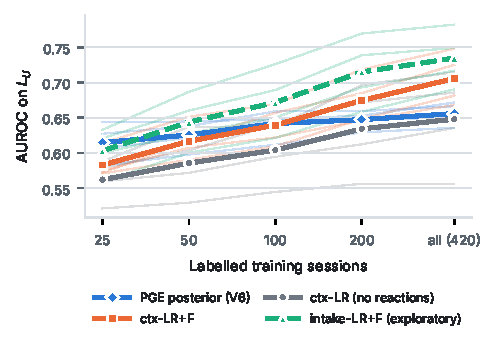
\includegraphics[width=\columnwidth]{figures/fig_lc.pdf}
\caption{Test AUROC on $\LU$ against the number of labelled training
sessions (mean over agents; thin lines: individual agents; identical
training subsets for every detector). Intake-LR+F is exploratory.}
\label{fig:lc}
\end{figure}

\begin{table}[t]
\centering
\caption{Registered hypotheses on $\LU$, pooled over
\val{C/derived/L_U/nagents} agents (stratified session bootstrap;
$^{*}$: 95\% CI excludes 0). H5 and H6 use oracle information
(Section~\ref{sec:exp-decomp}).}
\label{tab:hyp}
\setlength{\tabcolsep}{3pt}
\resizebox{\columnwidth}{!}{%
\begin{tabular}{llc}
\toprule
& Comparison & Estimate [95\% CI] \\
\midrule
H1 & AUROC(SelfCheckGPT) & \val{C/L_U/pooled/H1: AUROC(SelfCheckGPT)} \\
H1 & AUROC(semantic entropy) & \val{C/L_U/pooled/H1: AUROC(semantic_entropy)} \\
H2 & V6 $-$ V6$-$prior (feedback increment) & \val{C/L_U/pooled/H2: V6 - V6-prior} \\
H2b & ctx-LR+F $-$ ctx-LR (feedback increment) & \val{C/L_U/pooled/H2b: ctx_lr+fb - ctx_lr} \\
H3 & V6 $-$ ctx-LR & \val{C/L_U/pooled/H3: V6 - ctx_lr} \\
H4 & V6 $-$ SelfCheckGPT & \val{C/L_U/pooled/H4: V6 - SelfCheckGPT} \\
H4 & V6 $-$ semantic entropy & \val{C/L_U/pooled/H4: V6 - semantic_entropy} \\
H4b & ctx-LR+F $-$ SelfCheckGPT & \val{C/L_U/pooled/H4b: ctx_lr+fb - SelfCheckGPT} \\
H4b & ctx-LR+F $-$ semantic entropy & \val{C/L_U/pooled/H4b: ctx_lr+fb - semantic_entropy} \\
-- & V6 $-$ ctx-LR+F & \val{C/L_U/pooled/sec.: V6 - ctx_lr+fb} \\
H5 & $\eta_F-\bar\eta$ & \val{C/RA/pooled/H5: etaF (Bayes, feedback) - eta0 (Bayes, no feedback)} \\
H6 & V6-session $-$ LR-session+F & \val{C/RA/pooled/H6: V6-session - LR-session+fb} \\
\bottomrule
\end{tabular}}
\end{table}

\subsection{Where the information is}
\label{sec:exp-decomp}

\begin{table}[t]
\centering
\caption{Oracle-information analysis on $\LU$ (AUROC). $\bar\eta$: population
risk of the commitments; $\eta_\varnothing$: Bayes given the conversation the
agent saw (Theorem~\ref{thm:bound}'s bound for context-and-sample detectors);
$\eta_F$: Bayes given all reactions. V6-session and LR-session+F are told
which commitments are user-dependent in each session. Pooled differences
are in Table~\ref{tab:hyp}.}
\label{tab:decomp}
\setlength{\tabcolsep}{4pt}
\small
\begin{tabular}{lccccc}
\toprule
Agent & $\bar\eta$ & $\eta_\varnothing$ & $\eta_F$ & V6-sess. & LR-sess.+F \\
\midrule
Llama-70B & \tv{C/RA/70B/eta0 (Bayes, no feedback)} & \tv{C/RA/70B/etaX (Bayes, shown reactions)} & \tv{C/RA/70B/etaF (Bayes, feedback)} & \tv{C/RA/70B/V6-session} & \tv{C/RA/70B/LR-session+fb} \\
Llama-8B & \tv{C/RA/8B/eta0 (Bayes, no feedback)} & \tv{C/RA/8B/etaX (Bayes, shown reactions)} & \tv{C/RA/8B/etaF (Bayes, feedback)} & \tv{C/RA/8B/V6-session} & \tv{C/RA/8B/LR-session+fb} \\
Qwen-72B & \tv{C/RA/qwen/eta0 (Bayes, no feedback)} & \tv{C/RA/qwen/etaX (Bayes, shown reactions)} & \tv{C/RA/qwen/etaF (Bayes, feedback)} & \tv{C/RA/qwen/V6-session} & \tv{C/RA/qwen/LR-session+fb} \\
GPT-4o-mini & \tv{C/RA/gpt/eta0 (Bayes, no feedback)} & \tv{C/RA/gpt/etaX (Bayes, shown reactions)} & \tv{C/RA/gpt/etaF (Bayes, feedback)} & \tv{C/RA/gpt/V6-session} & \tv{C/RA/gpt/LR-session+fb} \\
Mistral-24B & \tv{C/RA/mistral/eta0 (Bayes, no feedback)} & \tv{C/RA/mistral/etaX (Bayes, shown reactions)} & \tv{C/RA/mistral/etaF (Bayes, feedback)} & \tv{C/RA/mistral/V6-session} & \tv{C/RA/mistral/LR-session+fb} \\
\bottomrule
\end{tabular}
\end{table}

Table~\ref{tab:decomp} and Figure~\ref{fig:ladder} locate the signal. \chk{The population risk
$\bar\eta$ alone is far above every sampling detector: much of $\LU$ is
visible in \emph{which} values an agent commits to, given the intake. The
user's reactions add $\eta_F-\bar\eta$ beyond it (H5). Almost all of that
information is already in the conversation the agent sees ($\eta_F-\eta_\varnothing$
is \val{C/RA/pooled/sec.: etaF (Bayes, feedback) - etaX (Bayes, shown reactions)}), so the failure of sampling detectors is not that the
information is absent from their input; it is that agreement between
resamples does not read it.} \chk{Given the same information (which commitments concern undisclosed
facts), the PGE posterior beats the supervised detector (H6), though by a
small margin whose interval nearly reaches zero
(\val{C/RA/pooled/H6: V6-session - LR-session+fb}). Registered without a claim: V6-session $-$ $\bar\eta$
is \val{C/RA/pooled/sec.: V6-session - eta0 (Bayes, no feedback)}, and the
reactions add \val{C/RA/range/LR-session+fb - LR-session} to LR-session across
agents.} Without that knowledge, V6 targets a schema-level set of
attributes that is only a proxy for the label's support, which costs it
\val{C/derived/V6session_gap/range} AUROC against V6-session, an order of
magnitude more than the H6 margin: knowing \emph{which} commitments concern
undisclosed facts matters far more than how the evidence is combined. A
deployable detector would have to learn this from labels, and with a few
hundred sessions it mostly does not: the exploratory intake-LR+F reaches
\val{X/L_U/range/intake_lr+fb}, against \val{C/RA/range/eta0 (Bayes, no feedback)}
for the population risk computed with the rules.

\begin{figure}[t]
\centering
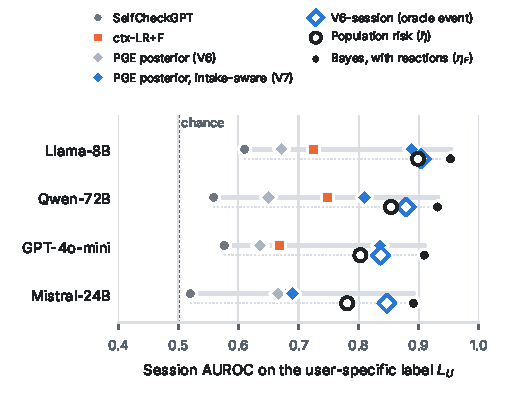
\includegraphics[width=\columnwidth]{figures/fig_ladder.pdf}
\caption{Where the signal is, on $\LU$. Sampling sits near chance; practical
detectors on PGE observables in the middle; the population risk
$\bar\eta$ and the Bayes posterior with reactions $\eta_F$ (oracle
information) bound what is achievable without and with the user.}
\label{fig:ladder}
\end{figure}

\subsection{A second domain}
\label{sec:exp-travel}

\begin{table}[t]
\centering
\caption{Second domain (travel booking), AUROC on $\LU$, 600 sessions per agent.}
\label{tab:travel}
\setlength{\tabcolsep}{3pt}
\resizebox{\columnwidth}{!}{%
\begin{tabular}{lcccccc}
\toprule
Agent & SelfCheck & ctx-LR & ctx-LR+F & V6 & $\bar\eta$ & $\eta_F$ \\
\midrule
GPT-4o-mini & \tv{T/L_U/gpt/SelfCheckGPT} & \tv{T/L_U/gpt/ctx_lr} & \tv{T/L_U/gpt/ctx_lr+fb} & \tv{T/L_U/gpt/V6} & \tv{T/RA/gpt/eta0 (Bayes, no feedback)} & \tv{T/RA/gpt/etaF (Bayes, feedback)} \\
Llama-8B & \tv{T/L_U/8B/SelfCheckGPT} & \tv{T/L_U/8B/ctx_lr} & \tv{T/L_U/8B/ctx_lr+fb} & \tv{T/L_U/8B/V6} & \tv{T/RA/8B/eta0 (Bayes, no feedback)} & \tv{T/RA/8B/etaF (Bayes, feedback)} \\
\bottomrule
\end{tabular}}
\end{table}

\chk{\pending{second-domain paragraph: does the pattern transfer (sampling
near chance, population risk large, reactions add, V6 vs supervised)?}}

\subsection{Natural-language reactions}
\label{sec:exp-patient}

\chk{The first simulated patient failed its gate. It contradicted 83\% of
wrong commitments and 79\% of correct ones (lift $1.06$; 100 sessions,
817 replies), against $75\%$ and $25\%$ for the noisy bit; the informed
variant, told the clinic's decision, did little better (97\% and 80\%, lift
$1.21$). Reading the replies shows why: the patient voiced doubt about facts
it had not been given, and the labeller counted doubt as contradiction. As
registered, neither was run at scale. A second version, registered before its data existed
(Amendment~5), uses GPT-4o-mini for both roles, lets the patient object only
to commitments that conflict with its listed facts, and labels a reply as a
contradiction only if it states a conflict.}
\chk{\pending{v2 audit (P(-1|wrong), P(-1|right), lift) and, if it passes,
detection V6 / V6-prior / ctx-LR / ctx-LR+F on both labels}} A simulated
user that does not track its own facts produces nearly uninformative
reactions; the gate is what keeps such a corpus out of the results.

\subsection{Choosing what to ask}
\label{sec:exp-loop}

The posterior's per-commitment risk $q_t$ is what chooses the question. On
confident user-dependent commitments in the test splits it predicts that
commitment's error with AUROC \val{X/PCQ/range/auroc_q} and expected
calibration error \val{X/PCQ/range/ece_q} across agents (exploratory; $q_t$
includes that commitment's own reaction).
\chk{\pending{measured clarification: posterior@1 vs no-question, random,
lowest-confidence; posterior@2 vs detailed questions and the full-rerun
control; questions per session; primary outcome wrong confident
user-dependent commitments}}

\subsection{Development-phase robustness}
\label{sec:exp-robust}

On the development corpora (protocol v2, before the display fix; label
$L$) we stress-tested the posterior by replacing the reactions seen by the
detectors (not the agent) with channels it does not assume: symmetric flips at $0.10$--$0.40$, asymmetric flips,
attribute-dependent noise, extra missingness, and a ``lazy'' user who
contradicts 60\% of wrong commitments and never confirms correct ones (labels
$L$, ten channels). The symmetric posterior V3 collapses under the lazy
user ($0.425$ for 70B, $0.576$ for 8B): it reads the absence of
confirmations as evidence of correctness. The general-channel V6 recovers
the channel from data and repairs this ($0.857$ and $0.855$). Across all ten
channels V6 has the best point estimate on both agents; with
session-clustered intervals its lead over the best baseline is significant
in six channels for 70B and two for 8B, so the robustness claim is about
consistency, not significance (``best baseline'' is the best of the
then-implemented baselines, chosen on test; ctx-LR was added later).
Regenerating reactions with the agent's trajectories fixed is the setting of
Theorem~\ref{thm:feedback}, and the posterior's AUROC falls monotonically
with the flip rate, as predicted ($0.890$, $0.793$, $0.690$ at
$\varepsilon=0.10$, $0.25$, $0.40$ for 70B). Structure-based detection does not help: graphon likelihoods score between $0.43$ and $0.58$ on every development corpus and label, even with the best variant chosen on test, and exact inference in a simple cascade model over the dependency graph (errors depend on attribute, bucket, and whether any parent is wrong) is no better than independence ($0.732$ vs.\ $0.734$ without value conditioning).

% ======================================================================
\section{Limitations}

\emph{Simulation.} The agents are real, but the patient is simulated: by a
noisy correctness bit in the main corpora and by an LLM in one corpus. The
oracle analyses rely on the simulator's known rules and prior, which a
deployment does not have. \emph{Two synthetic domains.} Both private-attribute domains are
simulators we designed, with deterministic rules and independent hidden
facts; real user populations have correlated, partially self-reported
facts.
\emph{Labels.} Labels are programmatic and noise-free by construction; there
is no human evaluation. \emph{Supervision.} The posterior and the supervised
baselines are fit on labelled training sessions; the posterior can run
without labels when the channel is known, which we only test in
development. \emph{Untested detectors.} A second model that reads the transcript with its
reactions is a feedback detector, not bounded by Theorem~\ref{thm:bound}; we
did not test one. Sampling detectors used three resamples (ten were
registered as optional and not run), and with exact matching semantic
entropy takes few values. We did not run hidden-state probes;
Theorem~\ref{thm:bound} predicts they share the within-context limit, but
they could exploit population risk as ctx-LR does. \emph{Theory.} Proposition~\ref{prop:posterior} is exact only under (A1)--(A2) with the true priors and channel, and the detector is a plug-in estimate; Theorem~\ref{thm:feedback} covers reactions regenerated for the detector with the agent's trajectories fixed, not the protocol's own noise, because the agent conditions on the reactions it is shown.

\section{Conclusion}

When an agent invents a fact about its user, its own samples cannot tell which of the users sharing its context it is wrong about. Some of the risk is visible in what the agent commits to; the rest is visible only through the user's reactions. Making the agent state
its assumptions as probabilistic commitments and recording the user's
reactions makes both available, and a Bayes analysis in a simulator with
known truth shows how much each is worth. \chk{\pending{one-sentence summary
of the confirmatory outcome for the posterior and for clarification}}

\paragraph{Reproducibility.} Code, all trajectories, the pre-registered
plan with its five amendments and a log of their commit times, every
analysis script, and a ledger of all runs including discarded variants are
at
\pending{anonymous repository link}.

\paragraph{Use of AI tools.} \pending{AI-assistance disclosure per ICAART
policy, without names.}

\bibliographystyle{plainnat}
\bibliography{refs,refs_extra}

\appendix
\section{Per-agent registered comparisons}
\label{app:peragent}

Table~\ref{tab:peragent} gives every registered difference per agent on both
labels (paired session-clustered bootstrap; $^{*}$: 95\% CI excludes 0).
H2: V6 $-$ V6$-$prior; H2b: ctx-LR+F $-$ ctx-LR; H3: V6 $-$ ctx-LR; H4: V6
$-$ SelfCheckGPT (SC) and semantic entropy (SE).

\begin{table*}[t]
\centering
\caption{Registered differences per agent (AUROC).}
\label{tab:peragent}
\scriptsize
\setlength{\tabcolsep}{3pt}
\begin{tabular}{lcccccc}
\toprule
Agent & H2 & H2b & H3 & H4 (SC) & H4 (SE) & V6$-$ctx-LR+F \\
\midrule
\multicolumn{7}{l}{\emph{User-specific label $\LU$ (primary)}} \\
Llama-70B & \val{C/L_U/70B/V6 - V6-prior} & \val{C/L_U/70B/ctx_lr+fb - ctx_lr} & \val{C/L_U/70B/V6 - ctx_lr} & \val{C/L_U/70B/V6 - SelfCheckGPT} & \val{C/L_U/70B/V6 - semantic_entropy} & \val{C/L_U/70B/V6 - ctx_lr+fb} \\
Llama-8B & \val{C/L_U/8B/V6 - V6-prior} & \val{C/L_U/8B/ctx_lr+fb - ctx_lr} & \val{C/L_U/8B/V6 - ctx_lr} & \val{C/L_U/8B/V6 - SelfCheckGPT} & \val{C/L_U/8B/V6 - semantic_entropy} & \val{C/L_U/8B/V6 - ctx_lr+fb} \\
Qwen-72B & \val{C/L_U/qwen/V6 - V6-prior} & \val{C/L_U/qwen/ctx_lr+fb - ctx_lr} & \val{C/L_U/qwen/V6 - ctx_lr} & \val{C/L_U/qwen/V6 - SelfCheckGPT} & \val{C/L_U/qwen/V6 - semantic_entropy} & \val{C/L_U/qwen/V6 - ctx_lr+fb} \\
GPT-4o-mini & \val{C/L_U/gpt/V6 - V6-prior} & \val{C/L_U/gpt/ctx_lr+fb - ctx_lr} & \val{C/L_U/gpt/V6 - ctx_lr} & \val{C/L_U/gpt/V6 - SelfCheckGPT} & \val{C/L_U/gpt/V6 - semantic_entropy} & \val{C/L_U/gpt/V6 - ctx_lr+fb} \\
Mistral-24B & \val{C/L_U/mistral/V6 - V6-prior} & \val{C/L_U/mistral/ctx_lr+fb - ctx_lr} & \val{C/L_U/mistral/V6 - ctx_lr} & \val{C/L_U/mistral/V6 - SelfCheckGPT} & \val{C/L_U/mistral/V6 - semantic_entropy} & \val{C/L_U/mistral/V6 - ctx_lr+fb} \\
Pooled & \val{C/L_U/pooled/H2: V6 - V6-prior} & \val{C/L_U/pooled/H2b: ctx_lr+fb - ctx_lr} & \val{C/L_U/pooled/H3: V6 - ctx_lr} & \val{C/L_U/pooled/H4: V6 - SelfCheckGPT} & \val{C/L_U/pooled/H4: V6 - semantic_entropy} & \val{C/L_U/pooled/sec.: V6 - ctx_lr+fb} \\
\midrule
\multicolumn{7}{l}{\emph{Composite label $L$ (secondary)}} \\
Llama-70B & \val{C/L/70B/V6 - V6-prior} & \val{C/L/70B/ctx_lr+fb - ctx_lr} & \val{C/L/70B/V6 - ctx_lr} & \val{C/L/70B/V6 - SelfCheckGPT} & \val{C/L/70B/V6 - semantic_entropy} & \val{C/L/70B/V6 - ctx_lr+fb} \\
Llama-8B & \val{C/L/8B/V6 - V6-prior} & \val{C/L/8B/ctx_lr+fb - ctx_lr} & \val{C/L/8B/V6 - ctx_lr} & \val{C/L/8B/V6 - SelfCheckGPT} & \val{C/L/8B/V6 - semantic_entropy} & \val{C/L/8B/V6 - ctx_lr+fb} \\
Qwen-72B & \val{C/L/qwen/V6 - V6-prior} & \val{C/L/qwen/ctx_lr+fb - ctx_lr} & \val{C/L/qwen/V6 - ctx_lr} & \val{C/L/qwen/V6 - SelfCheckGPT} & \val{C/L/qwen/V6 - semantic_entropy} & \val{C/L/qwen/V6 - ctx_lr+fb} \\
GPT-4o-mini & \val{C/L/gpt/V6 - V6-prior} & \val{C/L/gpt/ctx_lr+fb - ctx_lr} & \val{C/L/gpt/V6 - ctx_lr} & \val{C/L/gpt/V6 - SelfCheckGPT} & \val{C/L/gpt/V6 - semantic_entropy} & \val{C/L/gpt/V6 - ctx_lr+fb} \\
Mistral-24B & \val{C/L/mistral/V6 - V6-prior} & \val{C/L/mistral/ctx_lr+fb - ctx_lr} & \val{C/L/mistral/V6 - ctx_lr} & \val{C/L/mistral/V6 - SelfCheckGPT} & \val{C/L/mistral/V6 - semantic_entropy} & \val{C/L/mistral/V6 - ctx_lr+fb} \\
Pooled & \val{C/L/pooled/H2: V6 - V6-prior} & \val{C/L/pooled/H2b: ctx_lr+fb - ctx_lr} & \val{C/L/pooled/H3: V6 - ctx_lr} & \val{C/L/pooled/H4: V6 - SelfCheckGPT} & \val{C/L/pooled/H4: V6 - semantic_entropy} & \val{C/L/pooled/sec.: V6 - ctx_lr+fb} \\
\bottomrule
\end{tabular}
\end{table*}
\end{document}
